%%%%%%%%%%%%%%%%%%%%%%%%%%%%%%%%%%%%%%%%%%%%%%%%%%%%%%%%%%%%%%%%%%
%%%                      Homework _                            %%%
%%%%%%%%%%%%%%%%%%%%%%%%%%%%%%%%%%%%%%%%%%%%%%%%%%%%%%%%%%%%%%%%%%

\documentclass[letter]{article}

\usepackage{lipsum}
\usepackage[pdftex]{graphicx}
\usepackage[margin=1.5in]{geometry}
\usepackage[english]{babel}
\usepackage{listings}
\usepackage{amsthm}
\usepackage{amssymb}
\usepackage{framed} 
\usepackage{amsmath}
\usepackage{titling}

\usepackage{subcaption}
\usepackage{fancyhdr}

\pagestyle{fancy}


\newtheorem{theorem}{Theorem}
\newtheorem{lemma}{Lemma}
\newtheorem{definition}{Definition}

\newenvironment{menumerate}{%
  \edef\backupindent{\the\parindent}%
  \enumerate%
  \setlength{\parindent}{\backupindent}%
}{\endenumerate}







%%%%%%%%%%%%%%%
%% DOC INFO %%%
%%%%%%%%%%%%%%%
\newcommand{\bHWN}{7}
\newcommand{\bCLASS}{CS 189}

\title{\bCLASS: Homework \bHWN}
\author{William Guss\\26793499\\wguss@berkeley.edu}

\fancyhead[L]{\bCLASS}
\fancyhead[CO]{Homework \bHWN}
\fancyhead[CE]{GUSS}
\fancyhead[R]{\thepage}
\fancyfoot[LR]{}
\fancyfoot[C]{}
\usepackage{csquotes}

%%%%%%%%%%%%%%

\begin{document}
\maketitle
\thispagestyle{empty}

\begin{menumerate}
  \item \textbf{KMeans}
  \begin{menumerate}
  \begin{figure}
      \centering{
      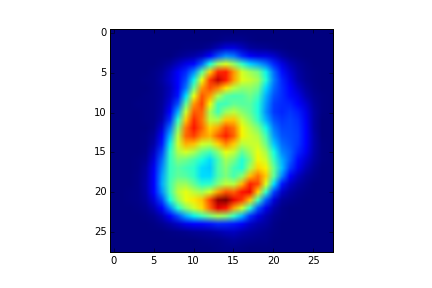
\includegraphics[height=0.3\textwidth]{class0.png}
      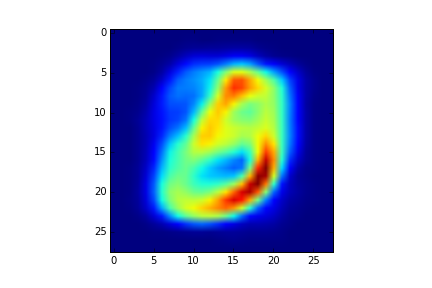
\includegraphics[height=0.3\textwidth]{class1.png}
      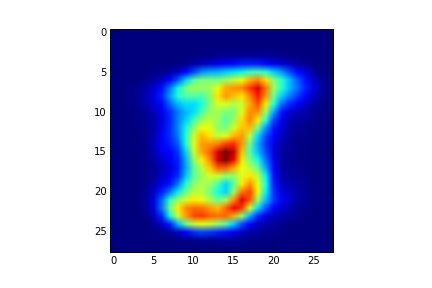
\includegraphics[height=0.3\textwidth]{class2.png}
      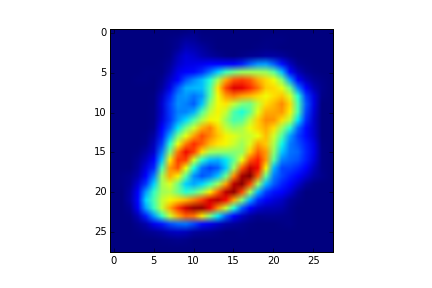
\includegraphics[height=0.3\textwidth]{class3.png}
      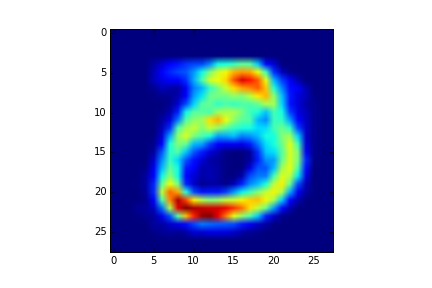
\includegraphics[height=0.3\textwidth]{class4.png}
      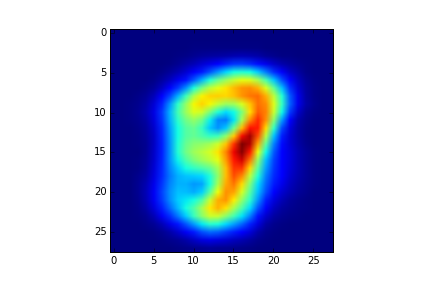
\includegraphics[height=0.3\textwidth]{class5.png}
      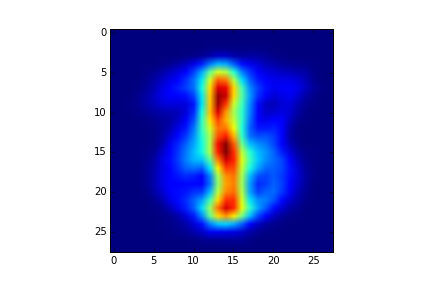
\includegraphics[height=0.3\textwidth]{class6.png}
      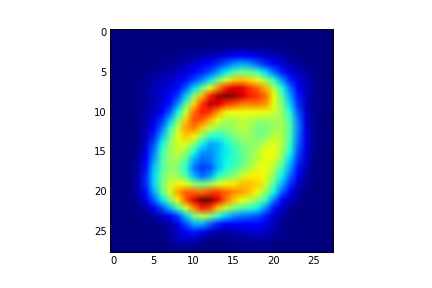
\includegraphics[height=0.3\textwidth]{class7.png}
      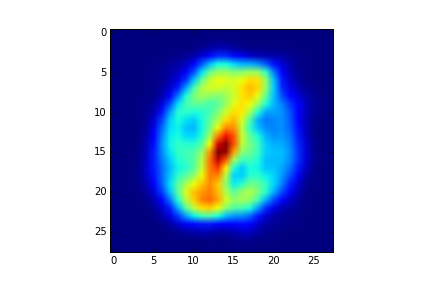
\includegraphics[height=0.3\textwidth]{class8.png}
      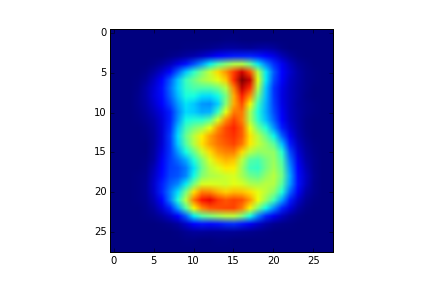
\includegraphics[height=0.3\textwidth]{class9.png}
        \caption{The mean centers of each class.}
      }

  \end{figure}
    \item After running $K$-Means Figure 1 is a sample plot of each class. Furthermore running $K$-means with different initializations leads to different loss; the classes are distributed differently each time.
  \end{menumerate}
  \item \textbf{Joke Recommender System}
  \begin{menumerate}
  \item \emph{Warm Up.} We tried the average value reccomendation system with some success! We got around 37\% error as seen in the iPython notebook. 
  \item \emph{$k$-NN.} We tried using $k$-NNS and below is a plot of the errors we received. $k$-NNs did best at $k=1000$. Awesome!

  \begin{center}
  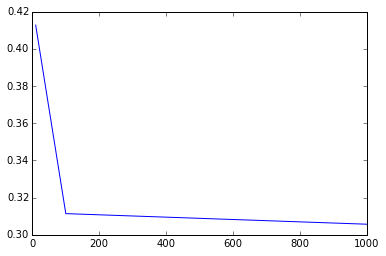
\includegraphics[width=0.5\textwidth]{knn_improve.png}
  \end{center}


    \item \emph{Latent Factor Model.} We apply the latent factor model by setting all the values in the matrix to $0$ where there are $NaN$s. We then perform SVD yeilding
  \begin{equation}
    R = USV^T,\;\;\;u_i = U_i,\;\;\;v_j = (SV^T)^T_j 
  \end{equation}
  Then we let $R_{ij} = \langle u_i, v_j \rangle$. Below is a plot of how well the MSE of this approximation does 
  with $S = diag(s_1, \dots, s_d, 0 \dots)$ as $d \to 100$.

  \begin{center}
  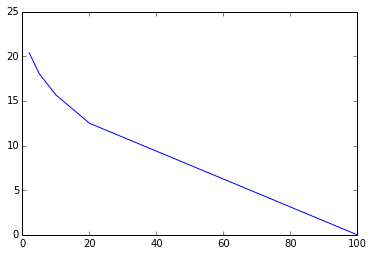
\includegraphics[width=0.5\textwidth]{training_svd.png}
  \end{center}

  Applying these approximations to the validation set we get the following graph indicating that $10$ latent dimensions optimizes
  the proper embedding of the data.

  \begin{center}
  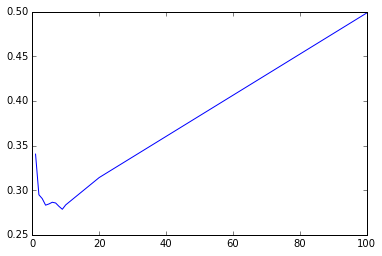
\includegraphics[width=0.5\textwidth]{index.png}
  \end{center}

  \item We will now attempt to do $L_1$ regularized gradient descent on the Frobenius MSE. Notice that $L(u_i, v_j)$ is symmetric
  in its calculation of the gradient so we skip the second derivations. First we calculate the gradient with respect to a single $u_i$.
  \begin{equation*}
    \begin{aligned}
        \frac{\partial L}{\partial u_i} &= \frac{\partial}{\partial u_i} \sum_{(k,l) \in S} (v^T_lu_k - R_{kl})^2 + \frac{\partial}{\partial u_i} \lambda \sum_{k=1}^d u_k^Tu_l \\
         &= \frac{\partial}{\partial u_i} \sum_{k \in S_1} \sum_{l \in S_2} (v^T_lu_k - R_{kl})^2 + 2 \lambda u_i  \\
         &= \frac{\partial}{\partial u_i} \sum_{l \in S_2} (v^T_lu_i - R_{il})^2 + 2 \lambda u_i  \\
         &= 2 \sum_{l \in S_2} (v_l^Tu_i - R_{il})v_l + 2 \lambda u_i  \\
     \end{aligned} 
  \end{equation*}
  Using the aforementioned symmetry we get
  \begin{equation}
    \begin{aligned}
        \frac{\partial L}{\partial u_i} &= \sum_{l \in S_2} (v_l^Tu_i - R_{il})v_l + \lambda u_i \\
        \frac{\partial L}{\partial v_j} &= \sum_{k \in S_1} (v_j^Tu_k - R_{kj})u_k + \lambda v_j 
    \end{aligned}
  \end{equation}

  Now we calculate the minimizers
  \begin{equation*}
  \begin{aligned}
   \frac{\partial L}{\partial u_i} = 0 &= \sum_{l \in S_2} (v_l^Tu_i - R_{il})v_l + \lambda u_i \\
   0 &= \lambda I u_i + \sum_{l \in S_2} (v_lv_l^Tu_i -  \sum_{l \in S_2}  v_lR_{il}  \\
   \sum_{l \in S_2}  v_lR_{il} &= \left(\lambda I + \sum_{l \in S_2} v_l\ocross v_l\right) u_i \\
   u_i &= \left(\lambda I + \sum_{l \in S_2} v_l\otimes v_l\right)^{-1} \sum_{l \in S_2}  v_lR_{il}
  \end{aligned}
  \end{equation*}
  This gives the following alternating minimizer method for every $i,j$ alternate the following.
  \begin{equation}
  \begin{aligned}
       u_i &= \left(\lambda I + \sum_{l \in S_2} v_l\otimes v_l\right)^{-1} \sum_{l \in S_2}  v_lR_{il} \\
       v_j &= \left(\lambda I + \sum_{k \in S_1} u_k\otimes u_k\right)^{-1} \sum_{l \in S_1}  u_kR_{kj}
    \end{aligned}  
  \end{equation}
  We implemented this in iPython and got the following results.
  \end{menumerate}
\end{menumerate}
%%%%%%% Be sure to set the counter and use menumerate

\end{document}